\documentclass[sigconf,authorversion,screen,microtype={protrusion=true,expansion,kerning,spacing}]{acmart}
\usepackage{amsmath}
\usepackage{mathtools}
\usepackage[english]{babel}
\usepackage{graphicx, lettrine}
\usepackage{calc}
\usepackage{bm}
\usepackage{epigraph}

\usepackage{pgfplots}
\pgfplotsset{compat=1.18}
\usetikzlibrary{backgrounds}

\copyrightyear{2026}
\acmYear{2026}
\setcopyright{cc}
\setcctype{by}
\acmConference[RecSys '26]{20th ACM Conference on Recommender Systems}{September 27-October 02, 2026}{Minneapolis, MN, USA}
\acmBooktitle{20th ACM Conference on Recommender Systems (RecSys '26), September 27-October 02, 2026, Minneapolis, MN, USA}
\acmDOI{10.1145/3773078.3831738}
\acmISBN{979-8-4007-2284-4/2026/09}

\begin{CCSXML}
<ccs2012>
   <concept>
       <concept_id>10002951.10003317.10003347.10003350</concept_id>
       <concept_desc>Information systems~Recommender systems</concept_desc>
       <concept_significance>500</concept_significance>
   </concept>
   <concept>
      <concept_id>10010270.10010271.10010272.10010275</concept_id>
      <concept_desc>Computing methodologies~Latent variable models</concept_desc>
      <concept_significance>500</concept_significance>
   </concept>
   <concept>
      <concept_id>10010270.10010281.10010290</concept_id>
      <concept_desc>Computing methodologies~Factorization methods</concept_desc>
      <concept_significance>500</concept_significance>
   </concept>
   <concept>
  <concept_id>10002951.10003317.10003347.10003350.10003351</concept_id>
      <concept_desc>Information systems~Collaborative filtering</concept_desc>
      <concept_significance>500</concept_significance>
   </concept>
   <concept>
       <concept_id>10003456.10003457</concept_id>
       <concept_desc>Social and professional topics~History of computing</concept_desc>
       <concept_significance>500</concept_significance>
   </concept>
</ccs2012>
\end{CCSXML}

\ccsdesc[500]{Information systems~Recommender systems}
\ccsdesc[500]{Computing methodologies~Latent variable models}
\ccsdesc[500]{Computing methodologies~Factorization methods}
\ccsdesc[500]{Information systems~Collaborative filtering}
\ccsdesc[500]{Social and professional topics~History of computing}

\keywords{Software archaeology, latent factors, low-rank matrix approximation, matrix factorization, sparsity, conjugate-gradient, cold start.}

\begin{document}

\title{EachMovie: archaeology of a first latent recommender system}
\author{John DeTreville}
\email{john@detreville.org}
\affiliation{
  \department{Systems Research Center (retired)}
  \institution{Digital Equipment Corporation}
  \city{Palo Alto}
  \state{California}
  \country{USA}
}

\begin{abstract}
This retrospective presents an ongoing archaeological reconstruction of EachMovie (1995--97), believed to be the first production-scale latent recommender system; it went live online a full decade before the Netflix Prize competition. Running on two office PCs, EachMovie gave its users highly personalized movie recommendations by computing 30-dimensional latent vectors from its evolving 2.8\;million-vote dataset (97.63\% sparse). Its Joint Quartic Polak-Ribi\`ere iterative solver converged rapidly and used a novel ``Unfilled'' objective function to overcome the inherent problems of zero- or mean-filled matrices. Its Early Voting data-augmentation strategy pre-loaded and stabilized the latent space every week by importing votes from professional reviews. EachMovie worked surprisingly well, cultivating a high degree of user engagement and trust, and noted movie critic Roger Ebert called it ``uncannily accurate.''
\end{abstract}

\maketitle{}

\section[``If you can name some movies you've liked~\ldots{}'']{\emph{\makebox[0pt][r]{``}If you can name some movies you've liked~\ldots{} we can name some others you might like too!''}}

\textbf{EachMovie} (1995--97) was an early research website designed, implemented, and operated at Digital Equipment Corporation's Systems Research Center (DEC SRC) that recommended movies to its users using latent-factor models of their tastes. These models were calculated in real time by a persistent \emph{Predictor} process as users added/\allowbreak{}changed/\allowbreak{}removed votes, and by a background \emph{Solver} process. EachMovie's goal was to create highly personalized movie recommendations for its users. Its calculations were quite involved for its time, but the results obtained were the state of the art.

I was the originator of and principal researcher for EachMovie from 1995 until leaving DEC in 1997. My SRC colleague Paul McJones took over until the project ended later in 1997.

Due to DEC's slow-motion collapse at the time, the lessons of EachMovie were never collected and published, leaving it literally prehistoric.\footnote{The final EachMovie dataset was subsequently available to the research community until 2004~\cite{HPLabs2004} and was widely used.} Mostly fragmentary artifacts remain~\cite{DeTrevillePatent2000} \cite{McJones97}, and some of their current owners are unclear. Even so, I have recently received a private cache of the original (noisy) datasets and assorted (inconsistent) source-file snapshots and others, and have used these in the ongoing reconstruction of EachMovie presented here. This work was aided by an AI-based analysis (using Google's Gemini~3 AI assistant~\cite{gemini2026}) to provide a firm foundation for this retrospective presentation.\footnote{AI assistance let me keep a cautious ethical/\allowbreak{}legal distance from the recovered artifacts. I am still working to obtain the permissions to share these more broadly.} I must emphasize, of course, that many portions of this paper are inescapably based solely on my own imperfect personal recollections, thirty years on.

\subsection{Research contributions}

This paper follows a strict archaeological reconstruction/\allowbreak{}audit of EachMovie's design/\allowbreak{}implementation/\allowbreak{}operation. The research contributions are threefold:

\begin{itemize}

    \item Reconstruction of the/a first latent recommender system. I document the architectural choices that let a pair of office PCs\footnote{With 133\;MHz Pentium processors, 64\;MiB / 96\;MiB RAM, and EIDE hard drives spinning at maybe 5400\,rpm.} compute 30-dimensional latent models from an evolving online dataset of 1,628 movies, 72,916 users, and 2,811,983 votes (97.63\% sparse).

    \item Implementation analysis of the Solver. I present the Joint Quartic error polynomial used with the Polak-Ribi\`ere con\-ju\-gate gradient (\textsc{cg}) solver to drive EachMovie's latent-factor search much more efficiently than the alternatives.

    \item Early Voting and expert seeding. I describe experience with the vote-import strategy using professional reviews to pre-load and stabilize EachMovie's latent geometries.

\end{itemize}

\section{The \textit{mise-en-sc{\`e}ne}}%
\label{section:SettingTheScene}

One of my chosen research directions in 1995 was, broadly stated, to discover better ways to ``find things,'' either on the Internet (as with the contemporaneous research on AltaVista~\cite{burrows2000altavista} at DEC SRC and sister labs in Palo Alto) or in the real world (as with movies).\footnote{EachMovie predated movies on the Internet. It included every movie in theatrical release in the US and Canada during its operation, as manually entered from websites and local newspapers, and from weekly photocopies from \textit{Variety}. Its DB also included many earlier movies in theatrical rerelease or in video release.}

During the design and implementation of EachMovie, I was often ignorant of related prior work and proceeded by engineering intuition to ``invent'' numerous useful techniques, many of which (it turns out) already existed. In this paper I use modern terminology to describe EachMovie, and highlight a few truly novel innovations.

My work was technically inspired by earlier Information Retrieval (\textsc{ir}) research at Bell Labs. Susan Dumais's work on \emph{Latent Semantic Indexing} (\textsc{lsi})~\cite{Dumais1988} inferred the semantics of documents from their textual contents. \textsc{lsi} constructed a matrix of $\textit{documents}\, \times \textit{words}$, counting the occurrences of each word in each document. Since the overall structure of this matrix was defined by relatively few latent factors, as expected from the \emph{effective rank} assumption, a low-rank approximation could capture (some/\allowbreak{}much of) the semantic ``signal'' of the documents' content. \textsc{lsi} used standard \emph{Singular Value Decomposition} (\textsc{svd})~\cite{Eckart1936} to factor its matrix into $U{\Sigma}V^\mathrm{T}$, then used the principal components for document retrieval. 

\section{``To infinity, \emph{and beyond!''}}

I decided EachMovie's user-movie vote matrix would also have low effective rank,\footnote{The \emph{actual} rank of a large $|U| \times |V|$ matrix is $\min(|U|, |V|)$ with high probability.} as with \textsc{lsi}, but devised a simpler rank-$K$ approximation $U_K V_K^\mathrm{T}$, where $U_K$ and $V_K$ held the \emph{non-orthonormal} user and movie latent vectors. (EachMovie chose $K = 30$.)\footnote{Too large a choice of $K$ can lead to overfitting. \textsc{svd} produces a \emph{unique} solution, but EachMovie's latent vectors were free to rotate/\allowbreak{}scale/\allowbreak{}shear in $K$-space, presumably reducing overfitting by allowing redundancies  in the latent factors.} The dot$\cdot$\allowbreak{}products of user vectors and movie vectors gave the predicted ratings.\footnote{Low-rank approximations let EachMovie treat similar movies as rough semantic synonyms. Just as \textsc{lsi} pulled \textit{film} and \textit{cinema} in a common direction, EachMovie brought together movies with related fans---and users with related tastes---performing a similar semantic decomposition. Our team briefly explored extending EachMovie to use higher-order tensors to model additional user inputs regarding multi-way interactions. One application was to be a \textit{Comments} feature to allow votes on other users' movie comments, with EachMovie choosing which to display; this was abandoned after deployment attracted toxic content (\emph{``so gay''}) that EachMovie could not yet adequately moderate automatically. Another feature, never begun, would have allowed user-authored personal movie axes (\textit{e.g.}, date-night \textit{vs} thriller), giving those users multiple votes per movie along these multiple axes.} 

It was my deliberate choice to build and operate EachMovie atop a mass-market PC hardware/\allowbreak{}software platform\footnote{Mass-market computers of that era were about $1000\times$ slower than today's.}, to help explore alternative platforms for SRC's research during a period of technological flux. While the theoretical foundations of EachMovie drew from \textsc{lsi}'s \emph{Big Math}, its implementation was strongly influenced by its own \emph{Small Iron}.

EachMovie's webserver called out to a persistent \emph{Predictor} as users added/\allowbreak{}changed/\allowbreak{}removed  votes; it cached all movie vectors in RAM and streamed user votes from a shared database. A background \emph{Solver} iterated over the database to update the latent vectors, pinging the Predictor every so often to trigger a refresh (\textit{e.g.}, every 90 minutes~/ thirty Solver iterations).

EachMovie's vote matrices were of course very sparse.\footnote{In \textsc{lsi}, most matrix entries are \emph{zero} since most documents don't contain most words (and vice versa). In EachMovie, most entries are \emph{missing} since most users haven't voted on most movies---which is \emph{very} different.} While it is easy to ``eliminate'' missing votes by zero-filling their empty matrix entries, EachMovie used a novel \textbf{Unfilled} objective function instead, where the objective function minimized the least-squares error exclusively for \emph{observed} votes:
\begin{equation}
E \;= \sum_{(i,j) \in \Omega} W_{ij} \; {\underbracket{(\text{Vote}_{ij} - \vec{u}_i \cdot \vec{v}_j) }_\text{observed-vote error}} ^ 2 \; + \; \lambda \, \underbracket{\Bigl( \sum_{i} ||\vec{u}_i||^2 + \sum_{j} ||\vec{v}_j||^2 \Bigr)}_{\text{\ensuremath{L_2} regularization}} \nonumber
\end{equation}
Here, $\Omega$ represents the observed-vote indices, and $\vec{u}$ and $\vec{v}$ are rows of $U_K$ and $V_K$. While this equation differs structurally from other formulations,\footnote{EachMovie's votes form a sparse bipartite graph, not a complete one. EachMovie Maxim\texttrademark{}: If your data don't fit some algorithm, change algorithms, not your data.} it had significant advantages, as shown in Section~\ref{section:SimulatedResults}. Ignoring missing votes protected niche signals from the ``gravity of the unknown'' inherent in artificially zero- or mean-filled \textsc{svd}.

User votes were input on a discrete scale of 0--5 stars but held internally on a scale of 0.0--1.0. The $W_{ij}$ vote weightings accommodated EachMovie's novel \textbf{Sounds Awful} votes.\footnote{EachMovie recorded ``Sounds Awful'' votes as 0 but with a reduced weighting of 0.2 to model vague negative signals---often based on trailers or hearsay---without overly distorting the surrounding latent geometries.} EachMovie set the $L_2$ regularization constant $\lambda = 2.0$ to eliminate numerical instability and avoid scaling to just denormals/\allowbreak{}infinities/\allowbreak{}NaNs.\footnote{Setting $\lambda = 2.0$ was the equivalent of $\lambda = 0.08$ on  the external 0--5 scale. The recovered source code sometimes names $\lambda$ as the constant \texttt{hundred}, providing archaeological evidence that $\lambda = 100$ was once tried too, perhaps with votes on EachMovie's earlier external scale of $\mathrm{F}^-$ to $\mathrm{A}^+$ that might have been manipulated on that same external scale. (Unfortunately, no revelatory comments/\allowbreak{}logs/\allowbreak{}documents remain.)}

This is a \textbf{Joint Quartic} polynomial over the users’ and movies’ latent factors, used to adjust all the latent factors at once, as guided by the global gradients. This differs from the quadratic-only \emph{Alternating Least Squares} (\textsc{als}) approach, which zigzags separately across the rows and columns. Born of my own na{\"i}ve design purity, this happy accident let the \textsc{cg} Solver navigate the 2,236,320-scalar landscape\footnote{EachMovie reached 72,916 users and 1,628 movies, with $K=30$, and the Solver was solving over $(|U| + |V|) \times K$ scalars.} about $20\times$ faster than \textsc{als}, also as shown in Section~\ref{section:SimulatedResults}.

EachMovie's Solver used the \emph{Polak-Ribi\`ere} (\textsc{pr}) variant of \textsc{cg} descent~\cite{shewchuk1994painless} instead of \emph{Fletcher-Reeves} (\textsc{fr}). \textsc{fr} can stagnate due to imperfect numerical results, while \textsc{pr}’s ability to reset if/\allowbreak{}when blown off course was crucial to EachMovie, as also shown below.

Local minima were not a problem for EachMovie. Modern optimization theory~\cite{Dauphinetal2014} suggests that typical higher-dimensional landscapes are dominated by saddle points rather than true local minima, helping gradient-based solvers avoid being trapped forever.

EachMovie was built around a classic positive-feedback loop: \textit{Votes~In} $\to$ \textit{Predictions~Out} $\to$ \textit{Votes~In}. EachMovie gained new users from word of mouth, and from some unexpected free advertising on AltaVista's landing page. Since many users of the era seemed to enjoy intensive online interactions, the EachMovie website design let them keep voting on and on for as many movies as desired.

\section{Early Voting and expert seeding}

New movies came out on Fridays. Their professional reviews were published on Thursdays, one day earlier.

To better support EachMovie's positive-feedback loop, a manual \textbf{Early Voting} strategy imported new reviews each Thursday. Professional reviewers became persistent \textit{pretend} users in EachMovie, with each new review imported as a pretend vote. This let EachMovie compute the new movies' latent vectors in time to recommend them to real users for Friday viewing.

Early Voting was part of a larger \emph{expert seeding} data-aug\-men\-ta\-tion strategy. Importing listicles of The Top 101 Movies Of All Time\texttrademark{} provided not just extra bonus votes, but also strengthened a semantic ``spine'' for the 30-D latent space. Even so, though professional reviewers can provide dense signals across a wide breadth of movies, it remains my belief that real users could do as useful a job of structuring the latent space \emph{in the long run}, meaning that these manual imports were needed only to get/\allowbreak{}keep the ball rolling.
I hope to test this hypothesis in future work.

\subsection{Roger Ebert and a cautionary tale}

% \epigraph{\raggedleft{} When you ask a friend if \textit{Hellboy} is any good, \\ you're not asking if it's any good compared to \textit{Mystic River}, you're asking if it's any good compared to \textit{The Punisher} \ldots{} If \\ \textit{Superman} is four, then \textit{Hellboy} is three and \textit{The Punisher} is two.}{``Shaolin Soccer,'' Roger Ebert, \textit{Chicago Sun-Times}, 2004}

When Roger Ebert called EachMovie ``uncannily accurate''~\cite{ebert1996critical}, it seemed like a major win,\footnote{I even designed self-congratulatory bumper stickers~\cite{BumperSticker1996} that our team mailed free to users on request.} but I soon worried it was all an unfortunate misunderstanding due to an unanticipated \textbf{Mirror} effect.

As described above, Early Voting and expert seeding imported numerous professional reviews into EachMovie, including several entered from the \emph{pretend} Roger Ebert. When the \emph{real} Roger Ebert then tried EachMovie IRL and found it so ``uncannily accurate,'' maybe he had simply glanced into an accidental Mirror and liked what he saw. That is, EachMovie might have been primed so as to adapt so quickly to the real Roger Ebert's own test votes, then provide such compelling recommendations right back, as to trick him into writing a better review than if EachMovie had not already imported a small yet representative body of his own reviews.

Or maybe not, of course, and it may be impossible to know so long after the fact. Still, imagining such practices \emph{did} somehow trigger too good a review for EachMovie, I offer my belated and posthumous apologies to the real Roger Ebert.

\section{User experiences}

In any case, EachMovie \emph{did} often seem uncannily accurate. Users were invited to write in, and many did:\footnote{Many of our respondents had never seen an automated recommender system before.}

\begin{itemize}
    \item \emph{Just wanted to slip out a quick note---this is a greatly enjoyable site! It has led us (my wife and myself) to some really great movie choices that we otherwise would have overlooked, but I guess that was the idea, wasn't it~:)}
  
    \item \emph{Well, last night I went out to the video store and rented a couple of movies that figured highly on my ``www.eachmovie.com'' prediction list. Amazing! One (\emph{Like Water for Chocolate}) was an absolute masterpiece~\ldots{} The other (\emph{Carrington}) I've rated as a 4!\;~\ldots{} You've got my attention! Let me congratulate you!}

      \item \emph{I've been using EachMovie for about a month now and, I have to admit, you are pretty good in your predictions. Not all the time, of course you're not God, but much of the time you're close.}

    \item \emph{I've been using it for two months, and it's eerily good at predicting what I'll like~\ldots{} One of my favorite games with EachMovie is to enter a bogus rating, just to see how it affects the predictions; when I revert to my true opinion, EachMovie recalculates all its predictions instantly.}

    \end{itemize}

I often repeated similar one-off experiments myself---add a single test user to EachMovie, vote on a single movie,\footnote{EachMovie's Unfilled objective function meant these test votes did not overly damage other users' or movies' latent vectors.} and see what happens---and the resulting predictive insights could be startling. Consider, for example, Jim Carrey, the popular/\allowbreak{}polarizing/\allowbreak{}prolific comic actor. As soon as such a test user voted up a single Jim Carrey movie, like \emph{The Mask}, EachMovie immediately recommended other Jim Carrey movies: \emph{Ace Ventura: Pet Detective}, \emph{Ace Ventura: When Nature Calls}, \emph{The Cable Guy}, \emph{Dumb and Dumber}, and so on. This impressed me since EachMovie contained \emph{no} ``Jim Carrey'' metadata, meaning the Jim Carrey effect was due \emph{solely} to latent factors.

EachMovie cultivated a high degree of user engagement. I was myself a particularly enthusiastic EachMovie user, recording a total of 465 votes over 20 months (1996--97).

\section{Neighborhood models}
\label{section:Other_approaches}

While contemporaneous systems like GroupLens~\cite{Resnick1994} \cite{konstan1997grouplens} from UMinn and Ringo/\allowbreak{}HOMR/\allowbreak{}Firefly~\cite{Shardanand1995} from the MIT Media Lab relied on $k$-nearest neighbor ($k$-\textsc{nn}) heuristics, EachMovie used latent factors. Neighborhood models seemed easy to compute but structurally shallow, failing to capture the transitive affinities that latent analysis so readily identifies. Also, neighborhood user-user models would seem \emph{far} more susceptible to the Roger Ebert Mirror effect than latent user-movie models like EachMovie's. Interestingly, Ebert found the $k$-\textsc{nn} recommender MovieCritic~\cite{Resnick1997}---primed with large amounts of professional criticism---to have a success rate ``comparable'' to EachMovie’s~\cite{ebert1996critical}, although it is possible this was largely due to the same hypothesized Mirror effect. (Gene Siskel was not as impressed with MovieCritic~\cite{Siskel1996}.)

% Additionally, of course, EachMovie avoided the \textit{Flaw of Averages} still found on most ratings websites, where % simple averages can so completely obscure polarized tastes and their correlations.

\section{From archaeology to re-animation}
\label{section:Re_animation}

The reconstruction now shifts from Dr.~Henry (``Indiana'') Jones,~Jr., to the methods of ``Dr.'' Henry Frankenstein.\footnote{Yes, Indiana Jones and Herr Frankenstein were both named ``Henry''~\cite{Spielberg1989} \cite{Whale1931}.}

\subsection{``Throw the switches!''}
\label{section:SimulatedResults}

To measure the Solver's performance, I simulated it on my M1 MacBook Pro laptop from 2020, along with a few alternative approaches. An AI-assisted rewrite into Python made this much more practical.

As described above, EachMovie used Polak-Ribi\`ere (\textsc{pr}) conjugate gradient descent. To test this choice, I also ran the Fletcher-Reeves (\textsc{fr}) \textsc{cg} option. Figure~\ref{fig:speeds} shows \textsc{pr} converging rapidly---almost $50\times$ faster than \textsc{fr}---as \textsc{pr}'s reset mechanism lets it navigate complicated geometries much more quickly.\footnote{These 2000 iterations would have taken over four days on EachMovie's original PC hardware from 1996. The simulated Solver ran over $100\times$ faster in Python on my more modern laptop from 2020, even slowed down by the various Python taxes.} Interestingly, an alternating \textsc{pr} performs \emph{almost} as poorly as \textsc{fr}.\footnote{For a fair comparison, each row-column pair counts here as a single iteration.}

\begin{figure}
\centering
\begin{tikzpicture}
  \begin{semilogxaxis}[
    xlabel={\emph{iteration (log-scale)}},
    ylabel={\emph{\small{``RMSE''} (0--5 stars)}},
    width=9cm,
    height=4.75cm,
    ymin=0, ymax=0.78,
    xmin=1, xmax=2001,
    legend cell align={left},
    legend style={
        fill=white, 
        fill opacity=0.9, 
        draw opacity=0, 
        text opacity=1,
        rounded corners=8pt,
        font=\tiny,
        at={(1.0,0.965)}, % Coordinates relative to axis (1,1 is top right)
        anchor=north east
    },
    legend image code/.code={
      \draw[mark repeat=2, mark phase=2] 
        (0cm,0cm) -- (0.3cm,0cm); % Default is usually 0.6cm or 2x
    },
    grid=both,
    grid style={line width=.1pt, draw=gray!10},
    major grid style={line width=.2pt,draw=gray!30},
    % Showing star increments on the y-axis
    ytick={0,0.2,0.4,0.6,0.8,1},
    yticklabels={0,1,2,3,4,5}
    ]

    \addplot[
    solid,
    color=ACMDarkBlue,
    sharp plot,
    mark size=1pt,
    line width = 1.2pt,
    opacity=0.75,
] table [x=iterations, y=rmse] {figure2_pr_data.dat}; \addlegendentry{Polak-Ribi{\`e}re}

\addplot[
    solid,
    color=ACMBlue,
    sharp plot,
    mark size=1pt,
    line width = 0.7pt,
    opacity=0.75,
] table [x=iterations, y=rmse] {figure2_fr_data.dat}; \addlegendentry{Fletcher-Reeves\!\!\!}

\addplot[
    densely dashed,
    color=ACMBlue,
    sharp plot,
    mark size=1pt,
    line width = 0.7pt,
    opacity=0.75,
    ] table [x=iterations, y=rmse] {figure2_als_data.dat}; \addlegendentry{alternating}

\addplot[
    loosely dotted,
    color=ACMRed,
    sharp plot,
    mark size=1pt,
    line width = 1pt,
    opacity=0.5,
    ] table [x=iterations, y=rmse] {figure2_svd_zero_data.dat};  \addlegendentry{(zero-filled)}

\addplot[
    densely dotted,
    color=ACMRed,
    sharp plot,
    mark size=1pt,
    line width = 1pt,
    opacity=0.5,
    ] table [x=iterations, y=rmse] {figure2_svd_mean_data.dat};  \addlegendentry{(mean-filled)}

\end{semilogxaxis}
\end{tikzpicture}

\caption{EachMovie's Polak-Ribi{\`e}re (\textsc{pr}) Solver performance across $\bm{2\times{}10^3}$ iterations, \textit{vs} alternatives.}
    \Description[EachMovie's Polak-Ribi\`ere Solver performance]{A graph showing the rapid Root-Mean-Square Error (``RMSE'') convergence of the Polak-Ribi\`ere (PR) solver used in EachMovie, following an initial transient. By comparison, the Fletcher-Reeves solver requires two orders of magnitude more iterations to converge. Zero- and mean-filled SVDs are included for comparison, and an \textsc{als} solver.}

\label{fig:speeds}
\end{figure}

All the iterative solvers perform better asymptotically than standard zero-filled \textsc{svd} or mean-filled \textsc{svd} (a fairer modern baseline that pretends each missing vote equals the overall mean). This suggests EachMovie's Unfilled objective function models its data better than \textsc{svd}, capturing more useful information.

Figure~\ref{fig:speeds} is provided only to compare the speeds of the iterative solvers; its \textit{Root-Mean-Square Error} \textsc{(rmse)} values are inaccurate since none of the votes were withheld, presumably leading to overfitting. There are many better ways to compute the \textsc{rmse}, of course, with varying strong points. Applying \emph{Leave-One-Out Cross-Validation} (\textsc{loocv})~\cite{Stone1974} to my own 465 votes (with permission) gives an \textsc{rmse} of 0.9767 stars.\footnote{Compared to 0.9568 at $K=20$ and 0.9499 at $K=25$, so $K=30$ was too large.} Figure~\ref{fig:giraffes} bins my votes---Sounds Awful, then 0--5 stars---plotted against their ascending \textsc{loocv} predictions, marking the movies at each quartile boundary.

\begin{figure}
  \centering
  \pgfplotsset{major tick length=0mm}

  \begin{tikzpicture}
  \begin{axis}[
      % xlabel={\emph{votes (sorted by range, then by prediction)}},
      % ylabel={\emph{predictions (0--5 stars)}},
      % axis line style={black!50, thin},
      width=9.6cm,
      height=7cm,
      ymin=0, ymax=5.8,
      xmin=0, xmax=465,
      clip=false, % Crucial for letting markers sit 'on top'
      grid=both,
      xmajorgrids=false,
      grid style={line width=.2pt, draw=gray!10},
      major grid style={line width=.2pt,draw=gray!30},
      % Customize the axis to show star increments
      xtick={20.5, 50.5, 88.5, 164.5, 278, 386.5, 449.5},
      xticklabels={{\color{ACMRed} ``\!$<$''}, {\color{ACMRed} $0\star$}, {\color{ACMRed} $1\star$}, {\color{ACMRed} $2\star$}, {\color{ACMRed} $3\star$}, {\color{ACMRed} $4\star$}, {\color{ACMRed} $5\star$}},
      x tick label style={font=\small, yshift=0pt},
      ytick={0, 1, 2, 3, 4, 5},
      yticklabels={$\color{ACMDarkBlue} 0.$, $\color{ACMDarkBlue} 1.$, $\color{ACMDarkBlue} 2.$, $\color{ACMDarkBlue} 3.$, $\color{ACMDarkBlue} 4.$, $\color{ACMDarkBlue} 5.$},
      y tick label style={font=\small},
      ticklabel style={/pgf/number format/fixed}, % Prevents scientific notation
      ]

\draw[color=ACMRed!50, line width = 0.65pt] (41, 0.055996366) -- (40, 2.417254718);
\draw[color=ACMRed!50, line width = 0.65pt] (60, 0.093102677) -- (59, 2.875384117);
\draw[color=ACMRed!50, line width = 0.65pt] (117, 0.533626578) -- (116, 3.500274515);
\draw[color=ACMRed!50, line width = 0.65pt] (212, 1.250319067) -- (211, 3.949895576);
\draw[color=ACMRed!50, line width = 0.65pt] (344, 0.859150862) -- (343, 5.204192155);
\draw[color=ACMRed!50, line width = 0.65pt] (429, 1.098262097) -- (428, 5.665289462);

  % 2. The LOO Predictions (Awful)
  \addplot[
      color=ACMDarkBlue,
      only marks,
      sharp plot,
      % mark size=1pt,
      line width = 1pt,
      opacity=0.75,
  ] table [x=index, y=predicted] {user1_loo_awful.dat};

  % 2. The LOO Predictions (0)
  \addplot[
      color=ACMDarkBlue,
      only marks,
      sharp plot,
      mark size=1pt,
      line width = 1pt,
      opacity=0.75,
  ] table [x=index, y=predicted] {user1_loo_0.dat};

  % 2. The LOO Predictions (1)
  \addplot[
      color=ACMDarkBlue,
      only marks,
      sharp plot,
      mark size=1pt,
      line width = 1pt,
      opacity=0.75,
  ] table [x=index, y=predicted] {user1_loo_1.dat};

  % 2. The LOO Predictions (2)
  \addplot[
      color=ACMDarkBlue,
      only marks,
      sharp plot,
      mark size=1pt,
      line width = 1pt,
      opacity=0.75,
  ] table [x=index, y=predicted] {user1_loo_2.dat};

  % 2. The LOO Predictions (3)
  \addplot[
      color=ACMDarkBlue,
      only marks,
      sharp plot,
      mark size=1pt,
      line width = 1pt,
      opacity=0.75,
  ] table [x=index, y=predicted] {user1_loo_3.dat};

  % 2. The LOO Predictions (4)
  \addplot[
      color=ACMDarkBlue,
      only marks,
      sharp plot,
      mark size=1pt,
      line width = 1pt,
      opacity=0.75,
  ] table [x=index, y=predicted] {user1_loo_4.dat};

  % 2. The LOO Predictions (5)
  \addplot[
      color=ACMDarkBlue,
      only marks,
      sharp plot,
      mark size=1pt,
      line width = 1pt,
      opacity=0.75,
  ] table [x=index, y=predicted] {user1_loo_5.dat};

% Indices for the Sounds Awful range
  \path (0, 0.01) node[draw=ACMDarkBlue, fill=white, fill opacity=1, inner sep=0.5pt, rounded corners=1.5pt]{\tiny $0$};
  \path (10, 0.36) node[draw=ACMDarkBlue, fill=white, fill opacity=1, inner sep=0.5pt, rounded corners=1.5pt]{\tiny $25$};
  \path (20, 0.70) node[draw=ACMDarkBlue, fill=white, fill opacity=1, inner sep=0.5pt, rounded corners=1.5pt]{\tiny $50$};
  \path (30, 1.04) node[draw=ACMDarkBlue, fill=white, fill opacity=1, inner sep=0.5pt, rounded corners=1.5pt]{\tiny $75$};
  \path (40, 2.42) node[draw=ACMDarkBlue, fill=white, fill opacity=1, inner sep=0.5pt, rounded corners=1.5pt]{\tiny $100$};

  % ZERO STARS:
  \path (41, 0.055996366) node[draw=ACMDarkBlue, fill=white, fill opacity=1, inner sep=0.5pt, rounded corners=1.5pt]{\tiny $0$};
  \path (45, 0.479596613) node[draw=ACMDarkBlue, fill=white, fill opacity=1, inner sep=0.5pt, rounded corners=1.5pt]{\tiny $25$};
  \path (50, 1.164598216) node[draw=ACMDarkBlue, fill=white, fill opacity=1, inner sep=0.5pt, rounded corners=1.5pt]{\tiny $50$};
  \path (55, 1.75868527) node[draw=ACMDarkBlue, fill=white, fill opacity=1, inner sep=0.5pt, rounded corners=1.5pt]{\tiny $75$};
  \path (59, 2.875384117 ) node[draw=ACMDarkBlue, fill=white, fill opacity=1, inner sep=0.5pt, rounded corners=1.5pt]{\tiny $100$};

  % ONE STAR
  \path (60, 0.093102677) node[draw=ACMDarkBlue, fill=white, fill opacity=1, inner sep=0.5pt, rounded corners=1.5pt]{\tiny $0$};
  \path (74, 1.052567609) node[draw=ACMDarkBlue, fill=white, fill opacity=1, inner sep=0.5pt, rounded corners=1.5pt]{\tiny $25$};
  \path (88, 1.421006514) node[draw=ACMDarkBlue, fill=white, fill opacity=1, inner sep=0.5pt, rounded corners=1.5pt]{\tiny $50$};
  \path (102, 2.29161565) node[draw=ACMDarkBlue, fill=white, fill opacity=1, inner sep=0.5pt, rounded corners=1.5pt]{\tiny $75$};
  \path (116, 3.500274515 ) node[draw=ACMDarkBlue, fill=white, fill opacity=1, inner sep=0.5pt, rounded corners=1.5pt]{\tiny $100$};

  % TWO STARS:
  \path (117, 0.533626578) node[draw=ACMDarkBlue, fill=white, fill opacity=1, inner sep=0.5pt, rounded corners=1.5pt]{\tiny $0$};
  \path (140, 2.010786256) node[draw=ACMDarkBlue, fill=white, fill opacity=1, inner sep=0.5pt, rounded corners=1.5pt]{\tiny $25$};
  \path (164, 2.491769791) node[draw=ACMDarkBlue, fill=white, fill opacity=1, inner sep=0.5pt, rounded corners=1.5pt]{\tiny $50$};
  \path (188, 3.007101518) node[draw=ACMDarkBlue, fill=white, fill opacity=1, inner sep=0.5pt, rounded corners=1.5pt]{\tiny $75$};
  \path (211, 3.949895576 ) node[draw=ACMDarkBlue, fill=white, fill opacity=1, inner sep=0.5pt, rounded corners=1.5pt]{\tiny $100$};

  % THREE STARS:
  \path (212, 1.250319067) node[draw=ACMDarkBlue, fill=white, fill opacity=1, inner sep=0.5pt, rounded corners=1.5pt]{\tiny $0$};
  \path (245, 2.677902329) node[draw=ACMDarkBlue, fill=white, fill opacity=1, inner sep=0.5pt, rounded corners=1.5pt]{\tiny $25$};
  \path (277, 3.030181749) node[draw=ACMDarkBlue, fill=white, fill opacity=1, inner sep=0.5pt, rounded corners=1.5pt]{\tiny $50$};
  \path (310, 3.405881376) node[draw=ACMDarkBlue, fill=white, fill opacity=1, inner sep=0.5pt, rounded corners=1.5pt]{\tiny $75$};
  \path (343, 5.204192155 ) node[draw=ACMDarkBlue, fill=white, fill opacity=1, inner sep=0.5pt, rounded corners=1.5pt]{\tiny $100$};

  % FOUR STARS:
  \path (344, 0.859150862) node[draw=ACMDarkBlue, fill=white, fill opacity=1, inner sep=0.5pt, rounded corners=1.5pt]{\tiny $0$};
  \path (365, 2.876089883) node[draw=ACMDarkBlue, fill=white, fill opacity=1, inner sep=0.5pt, rounded corners=1.5pt]{\tiny $25$};
  \path (386, 3.31063799) node[draw=ACMDarkBlue, fill=white, fill opacity=1, inner sep=0.5pt, rounded corners=1.5pt]{\tiny $50$};
  \path (407, 3.65398978) node[draw=ACMDarkBlue, fill=white, fill opacity=1, inner sep=0.5pt, rounded corners=1.5pt]{\tiny $75$};
  \path (428, 5.665289462 ) node[draw=ACMDarkBlue, fill=white, fill opacity=1, inner sep=0.5pt, rounded corners=1.5pt]{\tiny $100$};

  % FIVE STARS:
    \path (429, 1.098262097) node[draw=ACMDarkBlue, fill=white, fill opacity=1, inner sep=0.5pt, rounded corners=1.5pt]{\tiny $0$};
  \path (438, 3.257888927) node[draw=ACMDarkBlue, fill=white, fill opacity=1, inner sep=0.5pt, rounded corners=1.5pt]{\tiny $25$};
  \path (447, 3.610977395) node[draw=ACMDarkBlue, fill=white, fill opacity=1, inner sep=0.5pt, rounded corners=1.5pt]{\tiny $50$};
  \path (455, 3.819917116) node[draw=ACMDarkBlue, fill=white, fill opacity=1, inner sep=0.5pt, rounded corners=1.5pt]{\tiny $75$};
  \path (464, 5.788323968 ) node[draw=ACMDarkBlue, fill=white, fill opacity=1, inner sep=0.5pt, rounded corners=1.5pt]{\tiny $100$};

  \node[draw=gray!30, draw opacity=0, fill=white, fill opacity=0.7, text opacity=1, rounded corners=2pt, inner sep=3pt, font=\tiny, anchor=north west] at (axis cs:0, 5.8) {
    \begin{minipage}{5.5cm}
      \raggedright
      \emph{From the left:}
      ~
      \textbf{\color{ACMRed} Sounds Awful (``\!\boldmath{$<$}''):}~
      \textbf{0\%}~\textit{Flipper},
      \textbf{25\%}~\textit{Rent-a-Kid},
      \textbf{50\%}~\textit{Super Mario Bros.},
      \textbf{75\%}~\textit{[Yellow Dog]},
      \textbf{100\%}~\textit{[Tom Thumb]}.
      ~~
      %
      \textbf{\color{ACMRed} \boldmath{$0\star$:}}~
      \textbf{0\%}~\textit{Drop Zone},
      \textbf{25\%}~\textit{Hackers},
      \textbf{50\%}~\textit{Flintstones},
      \textbf{75\%}~\textit{Mr.\ Wonderful},
      \textbf{100\%}~\textit{Ghost in the Shell}.
      ~~
      %
      \textbf{\color{ACMRed} \boldmath{$1\star$:}}~
      \textbf{0\%}~\textit{Judge Dredd},
      \textbf{25\%}~\textit{La Scorta},
      \textbf{50\%}~\textit{Metro},
      \textbf{75\%}~\textit{Shadowlands},
      \textbf{100\%}~\textit{ST: Generations}.
      ~~
      %
      \textbf{\color{ACMRed} \boldmath{$2\star$:}}~
      \textbf{0\%}~\textit{Chain Reaction},
      \textbf{25\%}~\textit{MST3K},
      \textbf{50\%}~\textit{Dazed~\& Confused},
      \textbf{75\%}~\textit{Pretty Woman},
      \textbf{100\%}~\textit{It's a Wonderful Life}.
      ~~
      %
      \textbf{\color{ACMRed} \boldmath{$3\star$:}}~
      \textbf{0\%}~\textit{Rob Roy},
      \textbf{25\%}~\textit{Much Ado About Nothing},
      \textbf{50\%}~\textit{Sophie's Choice},
      \textbf{75\%}~\textit{Ben Hur},
      \textbf{100\%}~\textit{Toy Story}.
      $\swarrow$
    \end{minipage}
};

\node[draw=gray!30, draw opacity=0, text opacity=1, fill=white, fill opacity=0.0, rounded corners=2pt, inner sep=3pt, font=\tiny, anchor=south east] at (axis cs:465, 0) {
  \begin{minipage}{6cm}
    \raggedleft
    \textbf{\color{ACMRed} \boldmath{$4\star$:}}~
    \textbf{0\%}~\textit{Leaving Las Vegas},
    \textbf{25\%}~\textit{Around the World in 80 Days},
    \textbf{50\%}~\textit{Fantasia},
    \textbf{75\%}~\textit{When Harry Met Sally\ldots{}},
    \textbf{100\%}~\textit{Jurassic Park}.
    ~~~~~
    %
    \textbf{\color{ACMRed} \boldmath{$5\star$:}}~
    \textbf{0\%}~\textit{The Game}, \\
    \textbf{25\%}~\textit{Die Hard},
    \textbf{50\%}~\textit{Bringing Up Baby},
    \textbf{75\%}~\textit{The Maltese Falcon},
    \textbf{100\%}~\textit{Pulp Fiction}.
    \end{minipage}
};

\end{axis}
  \end{tikzpicture}

  \caption{My 465 votes, binned L-R by value then sorted L-R by \textsc{loocv} prediction, with quartile boundaries marked.}
  \Description{My own 465 votes on EachMovie, outlined for structural display. The votes are binned by value (Sounds Awful, then 0-star through 5-star), then sorted by the LOOCV-predicted value. These values are creatively plotted into seven ``giraffe curves,'' one illustrating each vote range; the horizontal axis lays out all of my 465 votes, as binned, while the vertical axis shows the LOOCV prediction for each. Each giraffe curve has five ovals reading (0), (25), (50), (75), and (100), marking the boundaries of each of this bin's quartiles. The center three ovals are normally close for higher bins, with a long tail extending above and below, but they display less elegantly in the lower bins. A legend (possibly screen-readable) names the movies I'd voted for in EachMovie (back in 1996--97) at each quartile boundary, within each vote range. For my Sounds Awful (``<'') bin, the quartile boundaries were: 0\% @ Flipper; 25\% @ Rent-a-Kid; 50\% @ Super Mario Bros.; 75\% @ Far From Home: The Adventures of Yellow Dog; and 100\% @ The Secret Adventures of Tom Thumb. Then, for my 0-star bin, the quartile boundaries were: 0\% @ Drop Zone; 25\% @ Hackers; 50\% @ The Flintstones; 75\% @ Mr.\ Wonderful; and 100\% @ Ghost in the Shell (Kokaku Kidotai). Next, for my 1-star bin, the quartile boundaries were: 0\% @ Judge Dredd; 25\% @ La Scorta; 50\% @ Metro; 75\% @ Shadowlands; and 100\% @ Star Trek: Generations. Continuing to my 2-star bin, the quartile boundaries were: 0\% @ Chain Reaction; 25\% @ Mystery Science Theater 3000: The Movie; 50\% @ Dazed and Confused; 75\% @ Pretty Woman; and 100\% @ It's a Wonderful Life (1946). Then, for my 3-star bin, the quartile boundaries were: 0\% @ Rob Roy; 25\% @ Much Ado About Nothing; 50\% @ Sophie's Choice (1982); 75\% @ Ben-Hur (1959); and 100\% @ Toy Story. For my 4-star bin, the quartile boundaries were: 0\% @ Leaving Las Vegas; 25\% @ Around the World in 80 Days (1956); 50\% @ Fantasia (1940); 75\% @ When Harry Met Sally... (1989); and 100\% @ Jurassic Park. Finally (!), for my 5-star bin, the quartile boundaries were: 0\% @ The Game (1997), released just before EachMovie shut down and which had only five recorded votes; 25\% @ Die Hard; 50\% @ Bringing Up Baby (1938); 75\% @ The Maltese Falcon (1941); and 100\% @ Pulp Fiction, along the latent Tarantino axis.}
  \label{fig:giraffes}
  \end{figure}

To add a more user-centered measure, I also performed a top-five precision audit across 100 randomized trials---withholding a different thirty of my votes each trial---resulting in a {\textit{Closed-Set Precision@5}} (P@5)~\cite{Manning2008} score of 65\%.\footnote{This audit counted only how many \emph{withheld} 4- or 5-star movies appeared in the resulting top-five predictions. I had 121 4- and 5-star votes, about 26\% of my total. My thirty votes withheld each trial were randomly selected from among \emph{all} my votes.} This is a $2.46\times$ lift compared to random chance, and a respectable value for a movie-recommender system from thirty years ago.

\subsection{``It's alive, \emph{it's alive!}''}

For a final proof of concept, I also resurrected EachMovie's webpage-generating code. Taking the Predictor's sorted dot$\cdot$\allowbreak{}products of users' latent vectors against their unseen movies', this code generates (Netscape-compatible) HTML for the user.\footnote{EachMovie's Web environment lacked CSS, cookies, JavaScript, and SSL.} (I performed portions of this simulation by hand.) Applied to my own EachMovie account, the whole patchwork assemblage generates the webpage shown in Figure~\ref{fig:Igor}. This is the first time EachMovie has run since being shut down late in 1997.

\begin{figure}
  \centering
  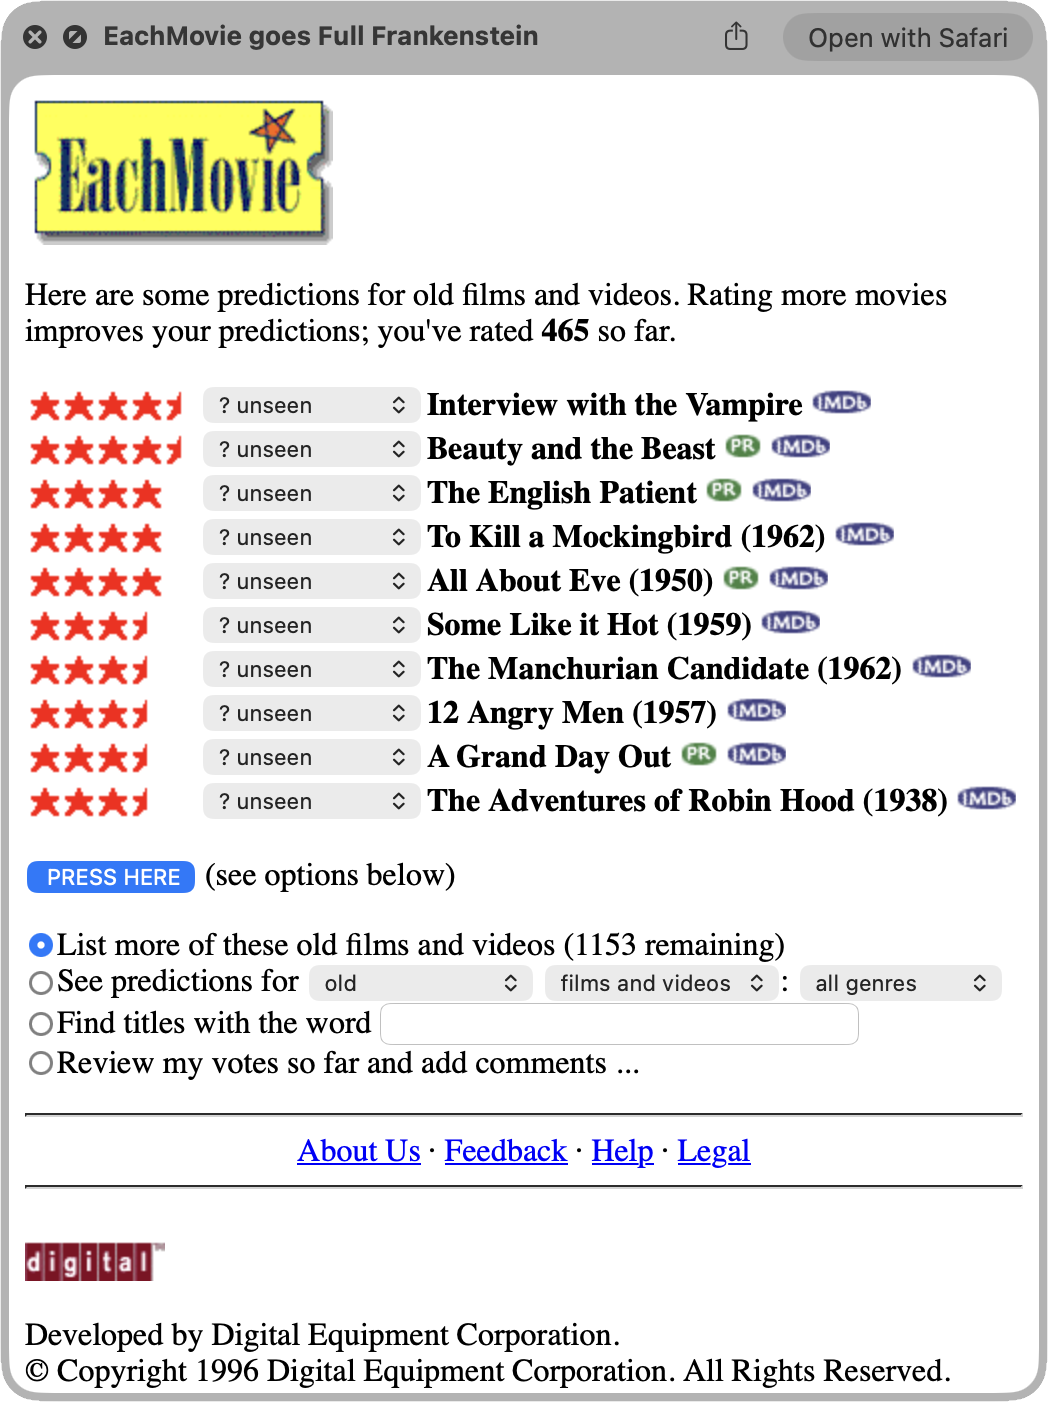
\includegraphics[width=0.88\linewidth]{resurrected.png}
  \caption[EachMovie redux]{The resurrected EachMovie, running with my own user account and its final dataset of movies and votes.}
  \Description[EachMovie redux]{A screenshot labeled ``EachMovie goes Full Frankenstein,'' showing the successfully re-animated restoration of EachMovie. The text is ``Here are some predictions for old films and videos. Rating more movies improves your predictions; you've rated 465 so far.'' followed by recommendations for \emph{Interview with the Vampire} \emph{[sic]}, with 4.687 stars predicted; \emph{Beauty and the Beast}, with 4.3395 stars predicted; \emph{The English Patient}, with 3.9015 stars predicted; \emph{To Kill a Mockingbird} (1962), with 3.801 stars predicted; \emph{All About Eve} (1950), with 3.7745 stars predicted; \emph{Some Like it Hot} \emph{[sic]} (1959), with 3.6995 stars predicted; \emph{The Manchurian Candidate}, with 3.634 stars predicted; \emph{12 Angry Men} (1957), with 3.6325 stars predicted; \emph{A Grand Day Out}, with 3.606 stars predicted; and \emph{The Adventures of Robin Hood} (1938), with 3.5965 stars predicted.}
\label{fig:Igor}
\end{figure}

\section{Back to the future}
\epigraph{\raggedleft{} And the end of all our exploring \\ Will be to arrive where we started \\ And know the place for the first time.}{\textit{Little Gidding}, T.S.~Eliot, 1942}

% \epigraph{\raggedleft{} People ask me why I write. I write to find out what I know.}{---commonly misattributed to Virginia Woolf}

Researchers have experimented with many architectures, but modern recommender systems have largely re-converged to the latent-factor foundations pioneered by EachMovie. Even with LLMs as sophisticated encoders for Two-Tower models, their latent embeddings feed into the same dot$\cdot$\allowbreak{}product geometries that EachMovie inferred on two office PCs.\footnote{Their Small Iron is now landfill, their  $\text{SiO}_2$ just dust, but the Big Math lives on.} EachMovie happened back when computation, cinema, and code could collide to form a purist system that can still seem ``uncannily accurate,'' thirty years on.

\begin{acks}
  Many thanks to Paul McJones for his work on EachMovie at SRC, for his archival guidance, and for reviewing drafts of this paper. Other reviewers included Julian McAuley (UCSD~CSE), Christine Seawell (UCI~English), Jerry Kuch (UWashington~CSE), and Mary-Claire van~Leunen~\cite{VanLeunen92}. %(Thanks also for van~Leunen's \textit{A Handbook for Scholars}~\cite{VanLeunen92}, invaluable in the preparation of this paper.)
Thanks also to Mike Looney, Vanessa Doherty, Carl Waldspurger, Mark Manasse, and Lyle Ramshaw for their work on EachMovie at SRC, to the Center for Open Science for hosting the permanent EachMovie repository~\cite{EachMovieOSF},\footnote{AUTHOR'S NOTE (TOO LATE): The EachMovie repository has moved to GitHub (\href{https://eachmovie.github.io}{eachmovie.github.io}) and Zenodo (\href{https://zenodo.org/communities/eachmovie/}{zenodo.org/communities/eachmovie/}).} and to T.S.~Eliot for inspiring the name ``EachMovie''~\cite{Eliot1917}.
\end{acks}

\bibliographystyle{ACM-Reference-Format}
\nocite{eliot1942littlegidding}
\bibliography{acmrecsys2026.bib}

\end{document}